% Preamble
% ---
\documentclass{article}

% Packages
% ---
\usepackage{amsmath} % Advanced math typesetting
\usepackage[utf8]{inputenc} % Unicode support (Umlauts etc.)
\usepackage{hyperref} % Add a link to your document
\usepackage{graphicx} % Add pictures to your document
\usepackage{listings} % Source code formatting and highlighting
\usepackage{framed} % Source code formatting and highlighting
\usepackage{appendix} % Source code formatting and highlighting
\usepackage[automake]{glossaries}

\usepackage[letterpaper, portrait, margin=1.5in]{geometry}

\graphicspath{ {images/} }

\newglossaryentry{sentinel}
{
    name={Sentinel},
    description={A Sentinel is a heuristic witnesses. It observes heuristics and vouches for the certainty and accuracy of them by producing temporal ledgers. The most important aspect of a Sentinel is that it produces ledgers that Diviners can be certain came from the same source by adding Proof of Origin to them}
}

\newglossaryentry{bridge}
{
    name={Bridge},
    description={A Bridge is a heuristic transcriber. It securely relays heuristic ledgers from Sentinels to Diviners. The most important aspect of a Bridge is that a Diviner can be sure that the heuristic ledgers that are received from a Bridge have not been altered in any way. The second most important aspect of a Bridge is that they add an additional Proof of Origin metadata}
}

\newglossaryentry{archivist}
{
    name={Archivist},
    description={An Archivist stores heuristics as a part of the decentralized data set with the goal of having all historical ledgers stored, but without that requirement. Even if some data is lost or becomes temporarily unavailable, the system continues to function, just with reduced accuracy. Archivists also index ledgers so that they can return a string of ledger data if needed. Archivists store raw data only and get paid solely for retrieval of the data. Storage is always free}
}

\newglossaryentry{diviner}
{
    name={Diviner},
    description={A Diviner answers a given question by analyzing historical data that has been stored by the XYO Network. Heuristics stored in the XYO Network must have a high level of Proof of Origin to determine the validity and accuracy of the heuristic. A Diviner obtains and delivers an answer by judging the witness based on its Proof of Origin. Given that the XYO Network is a trustless system, Diviners must be incentivized to provide honest analyses of heuristics. Unlike Sentinels and Bridges, Diviners use Proof of Work to add answers to the blockchain}
}

\newglossaryentry{gas}
{
    name={gas},
    description={The cost of a transaction (i.e. question) in the form of XYO Tokens}
}

\newglossaryentry{proof-of-origin}
{
    name={Proof of Origin},
    description={Proof of Origin is the key to verifying that ledgers flowing into the XYO Network are valid. A unique ID for source of data is not practical since it can be forged. Private Key signing is not practical since most parts of the XYO Network are difficult or impossible to physically secure, thus the potential for a bad actor to steal a Private Key is too feasible. To solve this, XYO Network uses Transient Key Chaining. The benefit of this is that it is impossible to falsify the chain of origin for data. However, once the chain is broken, it is broken forever and cannot be continued, rendering it an island}
}

\newglossaryentry{proof-of-work}
{
    name={Proof of Work},
    description={Proof of Work is a piece of data that satisfies certain requirements, is difficult to produce (i.e. costly, time-consuming), but easy for others to verify. Producing a Proof of Work can be a random process with a low probability of generation so that rigorous trial and error is required on average before a valid Proof of Work is created}
}

\newglossaryentry{bound-witness}
{
    name={Bound Witness},
    description={Bound Witness is a concept achieved by the existence of a bidirectional heuristic. Given that an untrusted source of data for the use of digital contract resolution (an oracle) is not useful, there is a substantial increase in certainty of the data provided by the establishment of such a heuristic. The primary bidirectional heuristic is proximity since both parties can validate the occurrence and range of an interaction by cosigning the interaction. This allows for a zero-knowledge proof that the two nodes were in proximity of each other.}
}

\newglossaryentry{smart-contract}
{
    name={smart contract},
    description={A protocol coined by Nick Szabo before Bitcoin, purportedly in 1994 (which is why some believe him to be Satoshi Nakamoto, the mystical and unknown inventor of Bitcoin). The idea behind smart contracts is to codify a legal agreement in a program and to have decentralized computers execute its terms, instead of humans having to interpret and act on contracts. Smart contracts collapse money (e.g. Ether) and contracts into the same concept. Being that smart contracts are deterministic (like computer programs) and fully transparent and readable, they serve as a powerful way to replace middle-men and brokers}
}

\newglossaryentry{cryptoeconomics}
{
    name={cryptoeconomics},
    description={A formal discipline that studies protocols that govern the production, distribution, and consumption of goods and services in a decentralized digital economy. Cryptoeconomics is a practical science that focuses on the design and characterization of these protocols}
}

\newglossaryentry{xyo-network}
{
    name={XYO Network},
    description={XYO Network stands for ``XY Oracle Network.'' It is comprised of the entire system of XYO enabled components/nodes that include Sentinels, Bridges, Archivists, and Diviners. The primary function of the XYO Network is to act as a portal by which digital smart contracts can be executed through real world geolocation confirmations}
}

\newglossaryentry{certainty}
{
    name={certainty},
    description={A measure of the likelihood that a data point or heuristic is free from corruption or tampering}
}

\newglossaryentry{accuracy}
{
    name={accuracy},
    description={A measure of confidence that a data point or heuristic is within a specific margin of error}
}

\newglossaryentry{oracle}
{
    name={oracle},
    description={A part of a DApp (decentralized application) system that is responsible for resolving a digital contract by providing an answer with accuracy and certainty. The term ``oracle'' originates from cryptography where it signifies a truly random source (e.g. of a random number). This provides the necessary gate from a crypto equation to the world beyond. Oracles feed smart contracts information from beyond the chain (the real world, or off-chain). Oracles are interfaces from the digital world to the real world. As a morbid example, consider a contract for a Last Will \& Testament. A Will''s terms are executed upon confirmation that the testator is deceased. An oracle service could be built to trigger a Will by compiling and aggregating relevant data from official sources. The oracle could then be used as a feed or end-point for a smart contract to call out to in order to check whether or not the person is deceased}
}

\newglossaryentry{heuristic}
{
    name={heuristic},
    description={A data point about the real world relative to the position of a Sentinel (proximity, temperature, light, motion, etc...)}
}

\newglossaryentry{transient-key-chain}
{
    name={Transient Key Chain},
    description={A Transient Key Chain links a series of data packets using Transient Key Cryptography}
}

\newglossaryentry{best-answer-score}
{
    name={Best Answer Score},
    description={A score generated by a Best Answer Algorithm that ranks the quality of the score.  The higher the score, the better it is, per the algorithm.  This score is used to determine which answer is better given two analyzed answers}
}

\newglossaryentry{best-answer-algorithm}
{
    name={Best Answer Algorithm},
    description={An algorithm used to generate Best Answer Scores when a Diviner chooses an answer.  The XYO Network permits the addition of specialized algorithms and allows the customer to specify which algorithm to use.  It is required that this algorithm will result in the same score when run on any Diviner given the same data set}
}

\newglossaryentry{origin-chain-score}
{
    name={Origin Chain Score},
    description={The score assigned to an Origin Chain to determine its credibility. This assessment takes length, tangle, overlap, and redundancy into consideration}
}

\newglossaryentry{origin-chain}
{
    name={Origin Chain},
    description={A Transient Key Chain that links together a series of Bound Witness heuristic ledger entries}
}

\newglossaryentry{origin-tree}
{
    name={Origin Tree},
    description={A data set of ledger entries taken from various Origin Chains to establish the origin of a heuristic ledger entry with a specified level of certainty}
}

\newacronym{pow}{PoW}{Proof of Work}

\newacronym{poo}{PoO}{Proof of Origin}

\newacronym{xy-oracle-network}{XY Oracle Network}{XYO Network}

\makeglossary

\title {XYO Network}
\author{Arie Trouw, Markus Levin, Scott Scheper}
\date{January 2018}

\begin{document}
\maketitle
\tableofcontents

\begin{center}
\line(1,0){50}
\end{center}

\begin{abstract}
Today, \glspl{smart-contract} are increasingly being used to execute contracts automatically, transparently and trustlessly. This, in effect, means lawyers, middlemen and escrow are unnecessary and may someday become obsolete. However, smart contracts have one key limitation: they rely in most cases on centralized data sources for data input. Additionally, there is often a limited offline application for them. To solve this limitation, we have developed the world's first location \gls{oracle} network which connects offline, trustless and decentralized location data with the blockchain and its smart contracts. We call this network the \Gls{xy-oracle-network}. Since its founding in 2012, the company behind the \Gls{xyo-network} has been steadily building a location network. The XYO Network makes it possible for smart contracts to plug into the real world by calling XY's network of devices that include not only XY's own devices but also other devices and products which are connected to the internet that can detect, record and/or relay location data. These connected elements, called \Glspl{sentinel}, are among other IoT devices like doorbells, cars, light bulbs, refrigerators, wireless routers, garage door openers, etc. as well as mobile apps,  phone and video cameras, etc. This network of devices can determine if an object is at a specific XY-coordinate at a given time. The use-cases and profound impact of such a technology are infinite.

The development of decentralized trustless applications has been gaining substantial momentum in recent years, and has now become generally accepted as an area for development and research in the field of Computer Science. Oracles are a significant portion of the power and infrastructure needs for decentralized applications, with most of the work revolving around the connectivity and aggregation of authoritative oracles. We believe that the need for a full featured, fully decentralized and trustless system of oracles is needed for decentralized applications to reach their full potential.

\begin{center}
\line(1,0){50}
\end{center}

\end{abstract}
\addcontentsline{toc}{section}{Application}
\section*{Application}
From straightforward to complex, the \Gls{xyo-network}'s usage  has vast applications that span a multitude of industries. Take for example an eCommerce Company that could offer its premium customers payment-upon-delivery services. To be able to offer this service, the eCommerce company would leverage the XYO Network and XY Platform (which uses XYO Tokens) to write a \gls{smart-contract} (i.e. on Ethereum's platform). The XYO Network could then track the location of the package being sent to the consumer along every single step of fulfillment; from the warehouse shelf to the the shipping courier, all the way into the consumer's house and every location in between. This could enable eCommerce retailers and websites to verify, in a trustless way, that the package not only appeared on the customer's doorstep, but also safely inside their home. Once the package has arrived in the customer's home (defined and verified by a specific XY-Coordinate), the shipment is considered complete and the payment to the vendor gets released. The eCommerce integration of the XYO Oracle Network thusly enables the ability to protect the merchant from fraud and ensure consumers only pay for goods that arrive in their home.

Consider an entirely different integration of the XYO Network with a hotel review site, whose current problem is that their reviews are often not trusted. Naturally, hotel owners are incentivized to improve their reviews at any cost. What if one could say with extremely high \gls{certainty} that someone was in San Diego, flew to a hotel in Bali and stayed there for two weeks, returned to San Diego, and then wrote a review about their hotel stay in Bali? The review would have a very high reputation, especially if it was written by a serial reviewer who has written many reviews with verified location data. The solutions the XYO Network can provide are infinite and the potential is unlimited.

\begin{center}
\line(1,0){50}
\end{center}

\section {System}
Create a trustless decentralized location \gls{oracle} network that is resistant to attack and produces the highest \gls{accuracy} and \gls{certainty} possible with the available data. Once a location oracle network is established, all other real-world \glspl{heuristic} can be accessed as oracle data, creating a full oracle system that provides the highest confidence and accuracy possible in a trustless, decentralized network.

\subsection {Problem}
With the advent of blockchain-based, trustless \glspl{smart-contract}, the need for \gls{oracle} services that arbitrate the outcome of a contract grows proportionately. Most current implementations of smart contracts rely on a single or aggregated set of authoritative oracles to settle the outcome of the contract. In cases where both parties can agree on the authority and incorruptibility of the specified oracle, this is sufficient. \textbf{However, in many cases, either an appropriate oracle does not exist or the oracle cannot be considered authoritative because of the possibility of error or corruption.}

Location oracles fall into this category. The divination of the location of a physical world item relies on the reporting, relay, storage, and processing components of the given oracle, all of which introduce error and can be corrupted. Risks include data manipulation, data pollution, data loss, and collusion. Thus the following problem exists:

Both \gls{certainty} and \gls{accuracy} of the location are negatively impacted by the lack of a trustless decentralized location oracle.

\subsection {Architecture}
The \Gls{xyo-network} has four primary components: \Glspl{sentinel}, \Glspl{bridge}, \Glspl{archivist}, and \Glspl{diviner}. Sentinels gather location \glspl{heuristic} via sensors, radios, and other means. Bridges take heuristics from Sentinels and provide them to Archivists. Archivists store heuristics for Diviners to analyze. Diviners analyze heuristics to generate answers to questions. This is accomplished using established advanced encryption and blockchain techniques and introduces the novel concept, \Gls{proof-of-origin}.

A single device may act as one or more of these four components of the system. Since topography, type of device and device optimization will impact the efficiency of each component, it would be rare, especially in a large XYO Network, that devices would be more than two of these components. Furthermore, a blockchain ledger that has more independent Proof of Origin will hold higher regard, so there is a natural penalty for a device acting as multiple components.


\subsection {Addressed by XYO Network}
The \Gls{xyo-network} provides location data and verification by addressing the following issues: trustlessness, accuracy, \gls{certainty}, cost, virtual security, and performance.

\subsection {Not Addressed by XYO Network}
The \Gls{xyo-network} does not address privacy, physical security, decentralized data storage, or network bridging. However, these are important to consider and will affect the implementation considerations when integrating or using XYO Network.

\subsection {Assumptions}
Edge devices on the \Gls{xyo-network} that produce and relay the needed location data are not physically secure, can be produced and added to the system at low cost, and are highly resource constrained.

\subsection {XYO Network's Four Components}

\subsubsection {Sentinels}
\Glspl{sentinel} are \gls{heuristic} witnesses. They observe heuristics and vouch for the \gls{certainty} and \gls{accuracy} of the heuristic by producing temporal ledgers. The most important aspect of a Sentinel is that it produces ledgers that \Glspl{diviner} can be certain came from the same source by adding \Gls{proof-of-origin} to them.

Given that \Gls{xyo-network} is a trustless system, Sentinels must be incentivized to provide honest heuristic ledgers. This is done by combining a reputation component with a payment component. A Sentinel is rewarded with XYO Network Tokens (XYO) when their heuristics are used to answer a question. To increase their odds of being rewarded, they must create heuristic ledgers that are consistent with their peers and provide Proof of Origin to identify themselves as the source of the heuristic.

Sentinels are usually off-line devices which either periodically go online or require \Glspl{bridge} to have their ledgers be part of the system.

\subsubsection {Bridges}
\Glspl{bridge} are \gls{heuristic} transcribers. They securely relay heuristic ledgers from \Glspl{sentinel} to \Glspl{diviner}. The most important aspect of a Bridge is that a Diviner can be sure that the heuristic ledgers that are received from a Bridge has not been altered in any way. The second most important aspect of a Bridge is that they add an additional \Gls{proof-of-origin}.

Given that \Gls{xyo-network} is a trustless system, Bridges must be incentivized to provide honest relaying of heuristics. This is done by combining a reputation component with a payment component. A Bridge is rewarded with XYO Network Tokens (XYO) when the heuristics that they relayed are used to answer a question. To increase their odds of being rewarded, they must create heuristic ledgers that are consistent with their peers and provide Proof of Origin to identify itself as the relay of the heuristic.

\subsubsection {Archivists}
\Glspl{archivist} store \glspl{heuristic} in a decentralized form with the goal of having all historical ledgers stored, but without that requirement. Even if some data is lost or becomes temporarily unavailable, the system continues to function, just with reduced \gls{accuracy}.

Archivists also index ledgers so that they can return a string of ledger data if needed.

Archivists store raw data only and get paid XYO Tokens solely for retrieval of the data and subsequent use. Storage is always free.

Archivists are networked, so asking one Archivist will result in that Archivist asking other Archivists for data that it does not contain. An Archivist can optionally store any ledger information that is returned to it. This will most likely result in two types of Archivists: ones that are at the data production edge of the ``cloud'' and the ones that are at the data consumption edge of the ``cloud''. Archivists in the middle will be hybrids. Each time data is handed off from one Archivist to another, additional \Gls{proof-of-origin} is appended in order to track payment, since all Archivists get paid. For a retrieval, a minimum Proof of Origin level can be set to increase validity.

The interests of \Glspl{sentinel}, \Glspl{bridge}, and Archivists must be aligned to prevent data bloat.

\subsubsection {Diviners}
\Glspl{diviner} answer a given question by analyzing historical data that has been stored by the \Gls{xyo-network}. \Glspl{heuristic} stored in the XYO Network must have a high level of \Gls{proof-of-origin} to determine the validity and \gls{accuracy} of the heuristic. A Diviner obtains and delivers an answer by judging the witness based on its Proof of Origin.

Given that the XYO Network is a trustless system, Diviners must be incentivized to provide honest analysis of heuristics. Unlike \Glspl{sentinel} and \Glspl{bridge}, Diviners use \Gls{proof-of-work} to add answers to the blockchain. Naturally, answers are prioritized by reward size, so the more XYO that is offered for an answer, the higher in priority the question would be.

In the case that the same question is asked more than once, more than one answer may be produced since the answer that is produced at a given moment is based on the available heuristics that the system can offer at that time.

Submitting an answer to the blockchain takes two steps. First, an analysis must be done to determine the best answer to a question. If multiple answers are generated by the system, then nodes will compare the answers and always choose the better answer. An example of a simple question would be: ``Where was a node on the network at a specific time in the past?''

\subsection {Choosing the Better Answer}
The Best Answer is the answer that has the highest validity score and has a higher \gls{accuracy} score than the minimum required accuracy. The validity score is based on the \Gls{origin-chain-score}. This does not provide absolute validity, only relative validity. The system will know what the highest record Origin Score was and that would be the 100 percent until a higher score is achieved, which then becomes the new 100 percent.

The \Gls{xyo-network} allows selection of the \Gls{best-answer-algorithm} for determining the Best Answer. This creates expansion for future research into alternative algorithms.

\begin{center}
\line(1,0){50}
\end{center}

\section {Origin Chains}
\Glspl{origin-chain} are the key to verifying that ledgers flowing into the \Gls{xyo-network} are valid. A unique ID for source of data is not practical since it can be forged. Private Key signing is not practical since most parts of the XYO Network are difficult or impossible to physically secure, thus the ability for a bad actor to steal a Private Key is too feasible. To solve this, XYO Network uses \Glspl{transient-key-chain}. The benefit of this is that it is impossible to falsify the chain of origin for data. However, once the chain is broken, it is broken forever and cannot be continued, rendering it an island. 

Every time a \gls{heuristic} ledger is handed off in XYO Network, the receiver appends their own \Gls{proof-of-origin}, which makes the Proof of Origin Ball bigger and generates a Proof of Origin Intersection. Proof of Origin Chains and Proof of Origin Intersections are the primary indicators used by \Glspl{diviner} to verify validity of ledgers. The equation for a Ledger Reputation is effectively what percent of the XYO Network was involved in making the Proof of Origin Ball associated with it. In theory, if 100 percent of the XYO Network records are linked with Proof of Origin and then fully analyzed, the odds of it being valid is 100 percent. If 0 percent of XYO Network records are available for analysis, then validity drops to 0 percent.

For added security, the Public Key for a Chain Link is not provided until the second entry for it is made available. This allows for the time interval between entries or other data to be added to the link.

\subsection {Origin Chain Score}
\Gls{origin-chain-score} is calculated as follows (default algorithm):

\begin{itemize}
\item PcL = \Gls{proof-of-origin} Chain Length
\item PcD = Proof of \Gls{origin-chain} Difficulty
\item Pc' Pc'' O = Proof of Origin Chain Overlap for Pc' and Pc''
\end{itemize}

\begin{equation*}\tag{1} \label{eq1}
Score = \prod_{i=0}^{i=n} \frac{PcL*PcD}{Pc' Pc'' O}
\end{equation*}

\subsection {Origin Tree}
An \Gls{origin-tree} is used to calculate the approximate validity of an answer. It uses the data gathered to generate an Ideal Tree, which is the tree that best fits that data for a given asserted answer. If Node N is located at X,Y,Z,T location, the error across all the data in the set must hold a certain value. To compute this error, we would calculate the MIN, MAX, MEAN, MEDIAN, and AVERAGE DISTANCE FROM THE MEAN.

The asserted answer that has the highest: [Difficulty * (1 - percent error)], is the Best Answer. Using the Proof of Origin Tree, we can identify and prune impossible branches.

\subsection {Reward for Diversity}
The \Gls{xyo-network}'s natural defense against team play is that it holds higher regard for a ledger with a more diverse \Gls{proof-of-origin}. For example, multiple \glspl{heuristic} that have Proof of Origin from the same sources are penalized while multiple heuristics that have diverse Proof of Origin are rewarded. This forces an attacker to have a number of devices so large that is is not economically viable.

\subsection {Privacy}
\Gls{xyo-network} stores all the Ledger Chains as public data in the \Glspl{archivist}. This creates the possibility of inferred data that is associated with people or things to be used nefariously.

\begin{center}
\line(1,0){50}
\end{center}

\section {XYO Token}
\begin{abstract}
The development of decentralized trustless applications has been gaining substantial momentum in recent years, and has now been established as an area for development and research in the field of Computer Science. \Glspl{oracle} are a significant portion of the power and infrastructure needs for decentralized applications, with most of the focus revolving around the connectivity and aggregation of authoritative oracles. We believe that the need for a full featured, fully decentralized and trustless system of oracles is needed for decentralized applications to reach their maximum potential.
\end{abstract}

\subsection {Economy of the Token}
The most fascinating notion at the center of cryptocurrency rests the concept of ``\gls{cryptoeconomics}.'' By implementing a Token or currency in one's platform, one can use cryptography to definitively prove past transactions. Then, through game theory and economics incorporated into the design of blockchain protocols, the system incentivizes actors to take the desired human behavior. Similar to how the Ethereum Platform's currency, Ether (ETH), is used as utility to compute and execute transactions, called ``\gls{gas},'' the \Gls{xyo-network} has its own currency, called the XYO Token (XYO). Using XYO, the XYO Network leverages cryptoeconomics to incentivize the desired behavior of providing accurate, reliable location \glspl{heuristic}. XYO Tokens can be thought of as``gas'' needed for one's smart contract to call out and travel through the real world in order to verify the XY-coordinate of a specified object.

The process works like this: A token holder queries the XYO Network by asking a question, (e.g.``Where is my Amazon package with XYO Address 0xe0EbD...e34a''). The question gets sent into a queue, where it waits to be processed and answered. Similar to how in Ethereum, one sets their Gas Limit and Gas Price, one can set their own XYO Gas Limit and XYO Gas Price. The higher one sets their XYO Gas Limit and XYO Gas Price, the higher priority their question will have in the queue. The XY Component that answers the query is the \Gls{diviner}. The cost of a question (in XYO tokens) is determined by the amount of data required to provide an answer to the query.  The more data needed, the more expensive the question and higher the XYO Gas Price. Potential queries to the XYO Network are infinite. For instance, a trucking and logistics company could query the XYO Network to ask, ``What is the location of every single car in our fleet?''

Once the XYO Token holder queries the XYO Network and pays the requested gas, the Diviner calls out to the relevant \Gls{archivist} to retrieve the pertinent data needed to answer the query. The data returned is derived from the \Glspl{bridge}, who originally gathered the data from the \Glspl{sentinel}. Sentinels are essentially devices or signals that verify the location of objects. These include devices like Bluetooth trackers, GPS trackers, geo-location tracking built into IoT devices, satellite tracking technology, QR-code scanners, RFID scanning and many others. XY Findables has pioneered and launched its consumer business, XY Find It, which has allowed it to test and process real-world location heuristics. All efforts of XY Find It have served to help significantly in designing the XYO Network Blockchain Protocol.

If the data provided by a Sentinel device (i.e. XY Find It Beacon) is used to answer a query, then all four Components involved in the transaction receive a part of the XYO Gas paid by the token holder: the Diviner (who searched for the answer), the Archiver (who stored the data), the Bridge (who transmitted the data) and the Sentinel (who recorded the location data)receive a part of the XYO Gas paid by the token holder. The distribution of the gas between the 4 components of the XYO Network always happens in the same proportion.  Within each component, gas gets distributed evenly.

\subsection {Beyond XY Find It Bluetooth \& GPS Tracking Sentinels}
The \Gls{xyo-network} is engaging with businesses to expand its network of \Glspl{sentinel} beyond its own network of XY Find It beacons, which total to over 800,000 globally as of January 2018. A variety of devices can act as Sentinels. Generally, the greater the Sentinel cardinality in the XYO Network, the more reliable the network. To broaden and strengthen the XYO Network, we are currently engaging mobile app companies, IoT companies and hardware companies to add Sentinels to the XYO Network. The XYO Network is providing solutions to a plethora of industries including eCommerce, government, automotive, healthcare, pharmaceutical, construction, insurance, utilities, oil \& gas, supply chain \& logistics, as well as businesses specializing in goods \& services reviews and traditional brick \& mortar retail. XY is working with a vast array of companies in order to create strategic partnerships that leverage \gls{cryptoeconomics} and economic incentives that are beneficial to both the Partner and end-user (which ultimately provide a cheaper product or service for the consumer).

\subsection {Token Generation Event - Main Sale}
The amount of XYO Tokens is finite and capped at the amount reached after the Token Generation Event Main Sale. When companies or individuals transmit a question to the \Gls{xyo-network}, they must be in possession of XYO Tokens to pay for the answer. Increased company participation in the network will call for a higher volume of XYO Tokens purchased to fulfill the increased query requests. Though the XYO Network economy would grow, the token amount is finite. After the conclusion of the Token Generation Event Main Sale, XY will aggressively pursue exchange listings at the largest and most liquid token exchanges to facilitate the XYO Network economy.

Please keep in mind that XYO Tokens do not represent equity. They are utility tokens used in blockchain-based \glspl{smart-contract} in order to access and transact with the XYO Network. If you are interested in buying equity in XY Findables, the company that has developed the XYO Network and operates both its blockchain business and its consumer Bluetooth and GPS tracking business (XY Find It), please refer to our SEC qualified and regulated Reg A+ equity sale.


\subsection {XYO Token Specifications}
\begin{itemize}
\item Smart contract platform: Blockchain Ethereum
\item Contract Type: ERC-20
\item Token: XYO
\item Token Name: \Gls{xyo-network} Utility Token
\item Token Address: 0x55296f69f40ea6d20e478533c15a6b08b654e758
\item Add the token to your ERC-20 compatible wallet (e.g. myEtherWallet, MetaMask, etc.) to view your XYO balance.
\item Total issuance: Finite and capped at the amount reached after the Token Main Sale
\item Amount issued during the main sale: Unlimited
\item Unsold and Unallocated tokens: Burned after the token sale event. No further XYO tokens will be generated after the Main Sale ends.
\end{itemize}

\subsection {Token Allocation}
For every token sold to the public, one token will be generated for the company XY Findables in order to ensure the development of the \Gls{xyo-network} platform and incentivize the company to grow the value of its network using traditional economics and \gls{cryptoeconomics}.
Initially, 3.2 billion tokens will be pre-generated for the company and team. See Fund Allocation (Figure 1.) for details.
\clearpage

\subsection {Fund Allocation}

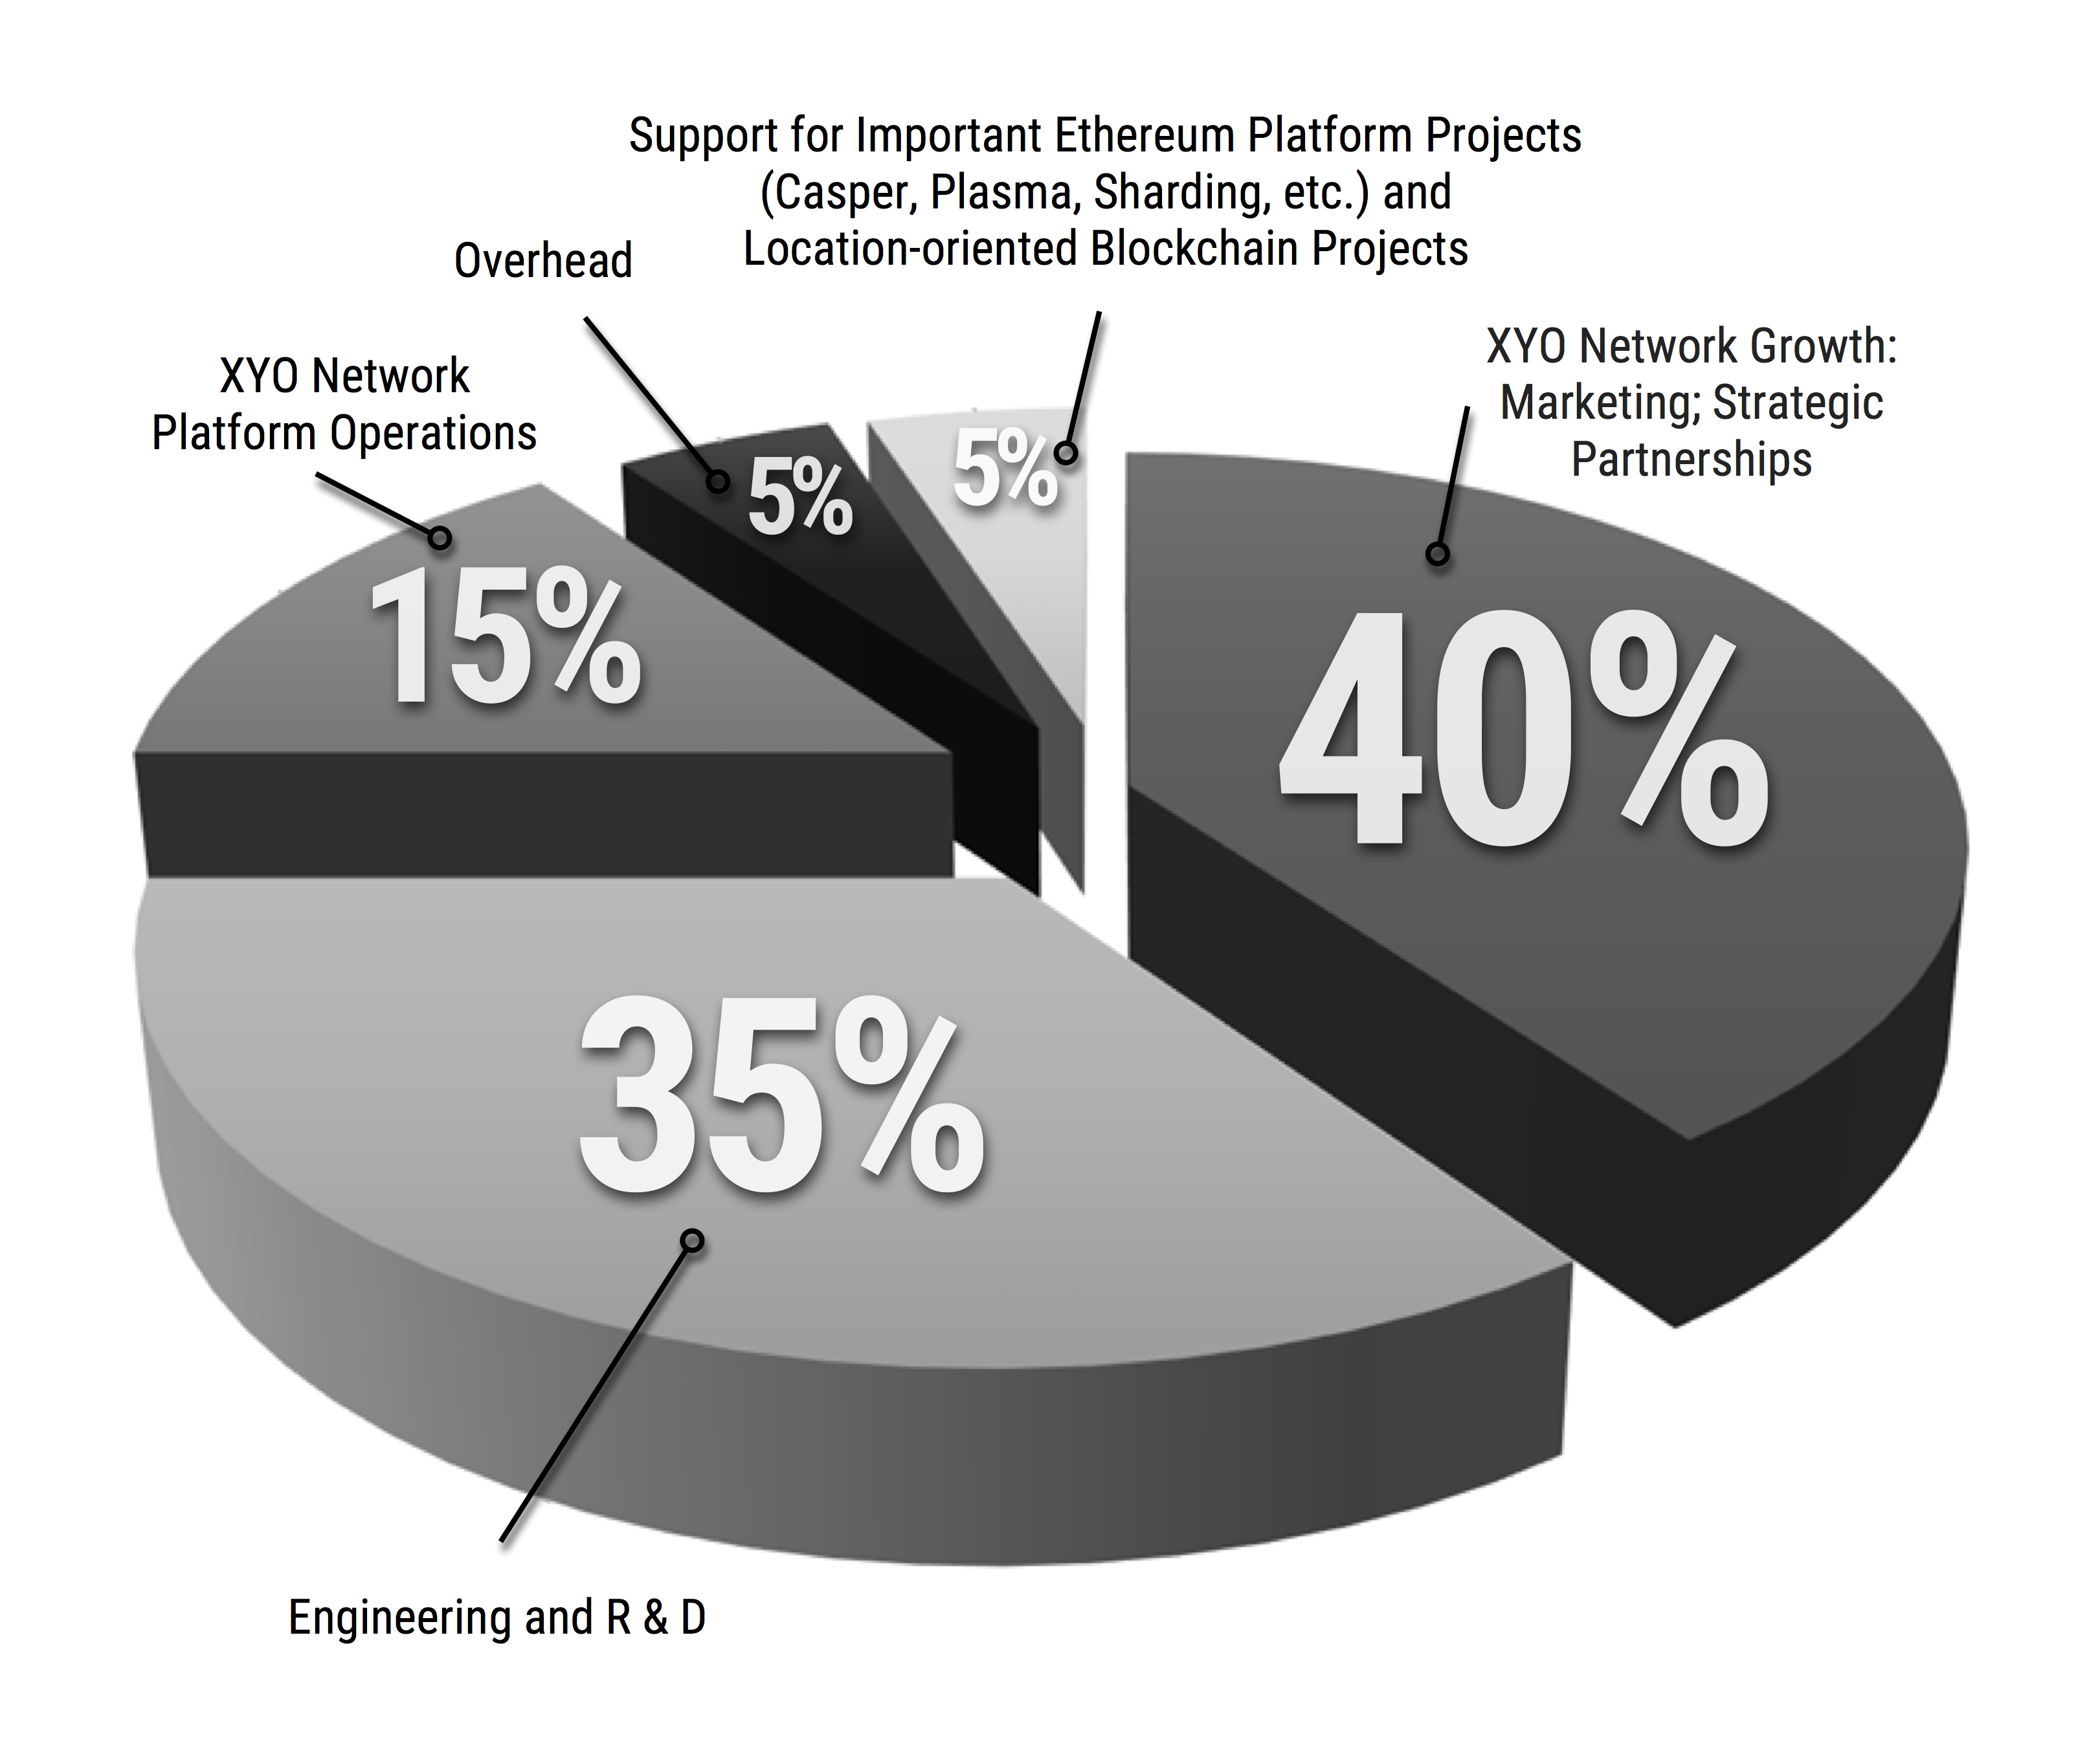
\includegraphics[width=\textwidth] {FundAllocationChart}
\begin{center}\textbf{Figure 1.}  Distribution of Funds
\end{center}

\begin{center}
\line(1,0){50}
\end{center}

\section {Bound Witness}
\begin{abstract}
Given that an untrusted source of data for the use of digital contract resolution (an \gls{oracle}) is not useful, we can substantially increase the \gls{certainty} of the data provided by first establishing the existence of a bidirectional \gls{heuristic}. The primary bidirectional heuristic is proximity since both parties can validate the occurrence and range of an interaction by cosigning the interaction. This allows for a zero-knowledge proof that the two nodes were in proximity of each other.
\end{abstract}

\subsection {Goal}
Determine the \gls{certainty} that an \gls{oracle} witness node in a trustless system gathered the data that it is sharing.

\subsection {Problem}
In a trustless system, a witness node can either by defect or corruption produce false data. Invalid data can be detected and removed simply if it falls outside the allowed range for that \gls{heuristic}. Valid but incorrect data (i.e. false data) is much more difficult to detect. 

\subsection {Unidirectional vs. Bidirectional Heuristics}
Most \glspl{heuristic} are unidirectional. This means that the element being measured cannot measure back, making heuristic data very difficult to validate. A bidirectional heuristic is one where the measured element measures back and reports on the other party which makes validation possible. Location is a rare heuristic in that it can be bidirectional with two edge nodes reporting on each other. A real-world example of this would be if two people who are near each other take a selfie, print a copy for each party, and then both sign the selfie, giving both parties Proof of Proximity. The only way for the two to have gotten this ``data'' would be for them to have been together.

\subsection {Network Effect}
Imagine a system where every edge node is expected to constantly produce these ``selfies'' as they travel around, and store them in a binder. They are also expected to keep that binder in time-sequential order and are never allowed to delete one. This establishes a proximity recorder for each edge node that can be cross referenced with the recorders of the other edge nodes.

\subsection {Non-Edge Nodes}
All nodes are considered ``witnesses'', including bridge, relay, storage, and analysis nodes. This allows for any data that is relayed from one node to the next to be bound. This is the concept of the \Gls{bound-witness}.

\subsection {Cross Reference}
Analyzing every set of ``selfies'' that is produced and chained together by every edge node allows the system to produce the Best Answer from the relative proximity of all the nodes that are in the network. If every node reports honestly and accurately, the mapping of all the relative positions of the edge nodes will achieve the maximum \gls{certainty} and \gls{accuracy} possible: 100 percent. Conversely, if every node either is dishonest or flawed, the certainty and accuracy both can approach the minimum of 0 percent.

Given a set of reported data and a query for a relative position of one of the edge nodes, an approximation of the position and a certainty and accuracy coefficient can be generated.

Given the same set of data and the same analysis algorithm, every calculation should arrive at the same position approximation and certainty and accuracy coefficients.

\subsection {Diagram}
S' and S'' (Figure 2.) are each a \Gls{sentinel} (edge node) that collect \glspl{heuristic}. When in contact with each other, they exchange heuristic data and public keys. Both build a full record of the interaction and sign the resulting interaction. That signed record then becomes the next entry in both of their local ledgers (16 for S' and 3 for S''). This action binds these two witnesses as being within proximity of each other.

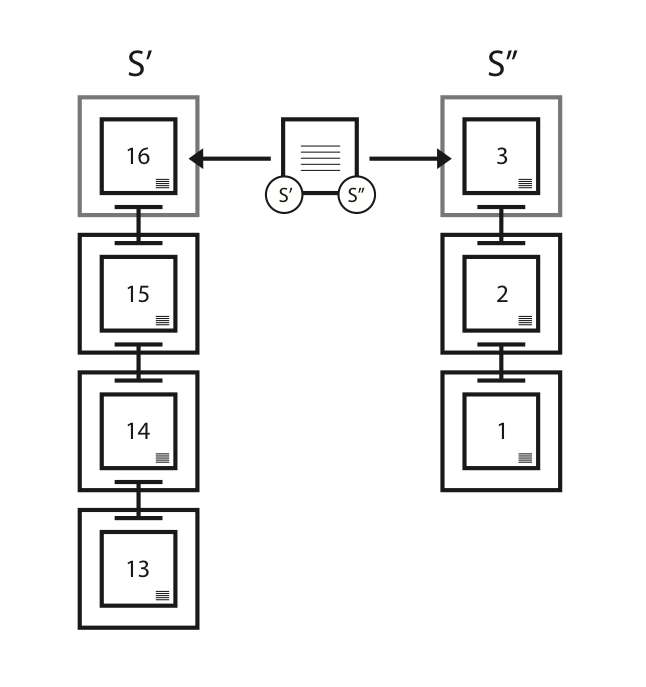
\includegraphics [width=\textwidth]{boundwitness}
\begin{center}\textbf{Figure 2.}  Record logging example between two Sentinels
\end{center}

\subsection {Summary}
Given a network of edge nodes that can collect signed, time-sequenced, bidirectional \glspl{heuristic}, a relative proximity between any two edge nodes can be established with a high level of confidence and \gls{accuracy}.

\begin{center}
\line(1,0){50}
\end{center}

\section {Proof of Origin}

\begin{abstract}
With a physical network comprised of untrusted nodes it is possible to determine the \gls{certainty} of data that has been provided by edge nodes based on a zero-knowledge proof that two or more pieces of data originated from the same source. Using these data sets combined with a number of similar data sets and the knowledge of at least one node's absolute location, the absolute location of the other node can be ascertained.
\end{abstract}

\subsection {Goal}
Verify that a set of \glspl{heuristic} come from the same origin within a trustless network.

\subsection {Problem}
In a trustless system, data may be lost, damaged, tampered with, or otherwise corrupted. This is the core assertion of the Byzantine Generals' Problem. Traditional \Gls{proof-of-origin} in a trustless system relies on a private key for signing transaction or contracts in a system. This works very well with the assumption that the node on the network that signs the data in question is physically and virtually secure. However, if the private key is compromised, then the ability to prove origin falters.

When applying trustless concepts to the Internet of Things, it must be assumed that edge nodes on the network are not physically or virtually secured. This brings forth the need to identify edge nodes without the use of unique IDs and to instead judge the data produced by them as being honest and valid without knowledge from outside the network.

\subsection {Basic Functionality}
Each origin maintains its own ledger and signs it to make a Proof of Origin Chain. Once information on the Proof of Origin Chain has been shared, it is effectively permanent. This is because the fork that happens after the share ends the chain and makes all future data from the witness to be treated as if it was from a new witness. To generate a link in a Proof of Origin Chain, the origin generates a public/private key pair. It then signs both the previous and next blocks with the same pair after including the public key in both blocks. Immediately after the signature is made, the private key is deleted. With the immediate deletion of the private key, the risk of a key being stolen or reused is greatly minimized.

\subsection {Transient Key Chaining}
A series of data packets can be chained together by using temporary private keys to sign two successive packets. When the public key paired with the private key is included in the data packets, the receiver can verify that both packets were signed by the same private key. The data in the packet cannot be altered without breaking the signature, assuring that the signed packets were not altered by a third party, such as a \gls{bridge} or storage node.

\subsection {Link Depth}
At a minimum, a node generates a new public/private key pair for every link in the Proof of Origin Chain, which has a Link Depth of 1. There may be N entries in the link table for a given Ledger Entry, with each entry specifying the distance in the future when part two of the link will be added. No two links may have the same order of magnitude on a base 2 scale. For example, [1,3,7,12,39] would be allowed, but [1,3,7,12,15] would not.

The depth 1 link is created, used and deleted when the previous block is published. However, links of depth greater than 1 have their pair generated as the previous block is being signed, and the second signing does not happen until N blocks later, after which the private key is deleted. For this reason, links of depth greater than 1 are always considered to be less secure than links of depth 1, but they can be used to improve performance and reduce data loss at the cost of that security.

\subsection {Fixed Order}
A key method for determining the sequence of ledgers is the order in which they were reported. Given that it is not possible for a device to change the order of any \Gls{proof-of-origin} signed ledger, an absolute order can be established by looking at all the Ledgers together.

\subsection {Second-to-Last Publishing}
A primary method for establishing \Gls{proof-of-origin} is the fact that a \Gls{sentinel} always reports its second to last block without reporting the last block. This allows the last block to have the signed link to its predecessor as evidence of the link.

\subsection {Empty Links}
To make a Proof of Origin Chain more secure, it is required that the chain is updated no more than once every ten seconds and no less than once every sixty minutes. In the case that no new data is available, an empty block will be added to the chain.

\subsection {Diagram}
As time travels from left to right (Figure 3.), the Proof of Origin Chain that is being built gets longer. At any given time, the producer of the chain will only provide the to the caller the entries with darkened borders, waiting for the second signing of the entry before making it available. For example, in the 3rd column, only entry 2 and 1 will be returned as being part of the chain.

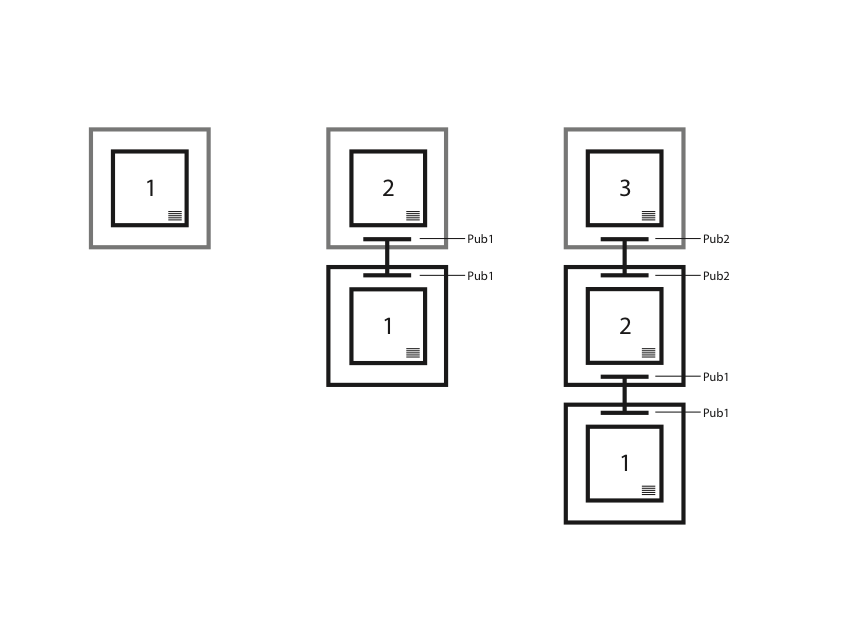
\includegraphics[width=\textwidth] {proofoforigin}
\begin{center}\textbf{Figure 3.}  Link inclusion example in a Proof of Origin Chain
\end{center}

\subsection {Summary}
Given a series of data packets that are signed in sequential pairs with temporary private keys and include the paired public keys, it can be determined with absolute \gls{certainty} that the packets came from the same origin.

\begin{center}
\line(1,0){50}
\end{center}
\clearpage

\section {XY Team}
XY's team is comprised of seasoned engineers, business development professionals and marketing experts. Arie Trouw solely founded XY Findables in 2012. Scott Scheper and Markus Levin joined as co-founders of the blockchain initiative in 2017 to assist in building the \Gls{xyo-network}.

\begin {framed}
\begin {center}
\textbf{Arie Trouw - Founder - Architect}\par
\end {center}
Ten years before Elon Musk wrote his first line of computer code, another young prodigy from South Africa was busy writing software on his TRS-80 Model I. In 1978, at the age of 10, Arie Trouw started developing software on the TRS-80 Model I, moving on to Atari, Apple, and PC. He then ran a series of bulletin boards centering on game-theory modification.

Arie is an accomplished serial entrepreneur with a rich history of technological breakthroughs and business successes involving multiple 8-figure exit events. He is a strong believer in decentralization and the creation of the integrated owner/user model. Arie founded XY in 2012 (incorporated as Ength Degree, LLC before it was converted to a C Corporation in 2016).

He currently serves as Chief Executive Officer, Chief Financial Officer, Chief Operating Officer and Chairman of the Board of Directors. Prior to starting XY-The Findables Company, Arie was CEO and Chairman of Pike Holdings Inc and Chief Technology Officer of Tight Line Technologies LLC. He received his Bachelor of Science in Computer Science from the New York Institute of Technology. Fun Fact: He is a member of one of the first Afrikaans speaking families to emigrate to the US from South Africa in 1976.

\end {framed}

\begin {framed}
\begin {center}
\textbf{Markus Levin - Co-Founder - Head of Operations}\par
\end {center}
Markus mined his first Bitcoin in 2013 and has been captivated by blockchain technologies ever since. Markus has over 15 years experience in building, managing and growing companies around the globe. Markus is originally from Germany (with English as his second language), and specializes in getting the most out of companies by implementing data-driven systems and utilizing the key talents of each employee to get the best out of his team.

After dropping out of his Ph.D. studies at Bocconi University, Markus began working with companies in hyper-growth industries around the globe. Markus has led cutting-edge technology ventures such as Novacore, ``sterkly'' (yes, with a lowercase ``s''), Hive Media and Koiyo.

\end {framed}

\begin {framed}
\begin {center}
\textbf{Scott Scheper - Co-Founder - Head of Marketing}\par
\end {center}
Scott has worked on many exciting ventures with extremely talented people including the Co-founder of Uber. Scott's first boss was Arie Trouw, who hired Scott in 2009 to join a company now operating as ``sterkly.'' What began as a Facebook app startup with 4 guys and a ping pong table, grew to a 200+ staff company with over 9-figures in revenue in less than two years.

In 2013 Scott took a break from corporate life to pursue the dream of working remotely on a laptop while sipping tropical drinks on the beaches of St. Thomas, Virgin Islands (U.S.). During this period, Scott launched Greenlamp, a programmatic advertising agency specializing in direct-response paid advertising. The agency was fully automated; built entirely using automated systems to manage the advertising campaigns. The team consisted of part-time software engineers, with its only full-time employee being Scott. The advertising campaigns were managed by an automated rule system, nicknamed ``Stewie'' (after the Family Guy character).Twenty-four hours a day, Stewie managed advertising campaigns, making automated tweaks and even emailed Scott to chat about the changes made (Stewie's emails also included signature Stewie lines). In its first year, Greenlamp generated 8 figures in revenue.

When not optimizing marketing campaigns or engrossing himself in the world of blockchain technologies, Scott can be found studying reading books about his idols, Gary C. Halbert and Charlie Munger or spending time with friends and family in San Diego, California.

\end {framed}

\begin {framed}
\begin {center}
\textbf{Wiliam Long - Co-Founder - Head of Hardware}\par
\end {center}
William is a veteran computer hardware and firmware technologist with over 25 years experience in engineering management and electrical engineering development. He's also a successful entrepreneur, having founded several computer product and data storage companies, some of which have become publicly traded. William has authored 3 US patents, and is an iOS/OSX product development authority (as an Apple certified developer since 1986).

He is a rare breed that spends his free time programming Bluetooth and GPS hardware, preferring to do soin Assembly code. William brings considerable expertise in Storage Area Networks (SANs), NAS systems, and enterprise class data storage systems for mission-critical applications (such as eCommerce and medical data storage).

He received his Bachelor of Science in Electrical Engineering from Northrop University in Inglewood, California, and is one of Cisco's top certified networking recommendations.

\end {framed}

\subsection{Additional Team Members}
\begin {framed}
\begin {center}
\textbf{Christine Sako - Head of Analytics}
\end {center}
\end {framed}

\begin {framed}
\begin {center}
\textbf{Johnny Kolasinski - Head of Media}
\end {center}
\end {framed}

\begin {framed}
\begin {center}
\textbf{Jordan Trouw - Head of Customer Experience}
\end {center}
\end {framed}

\begin {framed}
\begin {center}
\textbf{Lee Kohse - Head of Design}
\end {center}
\end {framed}

\begin {framed}
\begin {center}
\textbf{Louie Tajeda - Head of Warehouse Logistics}
\end {center}
\end {framed}


\begin {framed}
\begin {center}
\textbf{Maria Cornejo - Head of Retail Management}
\end {center}
\end {framed}

\begin {framed}
\begin {center}
\textbf{Maryann Cummings - Head of Support}
\end {center}
\end {framed}

\begin {framed}
\begin {center}
\textbf{Patrick Turpin - Head of Hardware QA}
\end {center}
\end {framed}

\begin{center}
\line(1,0){50}
\end{center}

\section {Advisors}
The \Gls{xyo-network} is fortunate to count a varied group of advisors to its roster of experts.

\begin{center}
\line(1,0){50}
\end{center}

\clearpage
 
\printglossaries

\end{document}
